\section{CASO DE USO: ÁRVORE BINÁRIA DE PESQUISA}

O Código \ref{listing:abp} abaixo demonstra a instanciação de uma árvore binária de pesquisa, os detalhes da implementação
serão discutidos adiante. O objetivo em um primeiro momento é demonstrar a facilidade de usar implementações funcionais
sobre a árvore afim de realizar algumas operações comuns.

\begin{listing}[H]
    \begin{minted}[linenos,xleftmargin=2mm,tabsize=2,breaklines,autogobble,numbersep=5pt]{python}
    from Btree import BinaryTree, Node
    from toolz import compose, compose_left
    
    tree = BinaryTree([ 5, 2, 6, 10, 1, 3, 4, 9 ])
    \end{minted}
    \caption{Árvore Binária de Pesquisa}
    \label{listing:abp}
\end{listing}

Nota-se na linha 4 que a árvore \textbf{tree} é criada a partir de uma lista de inteiros.
As inserções destes inteiros produzem a árvore representada na Figura \ref{fig:btree}:

\begin{figlisting}[H]
    \centering
    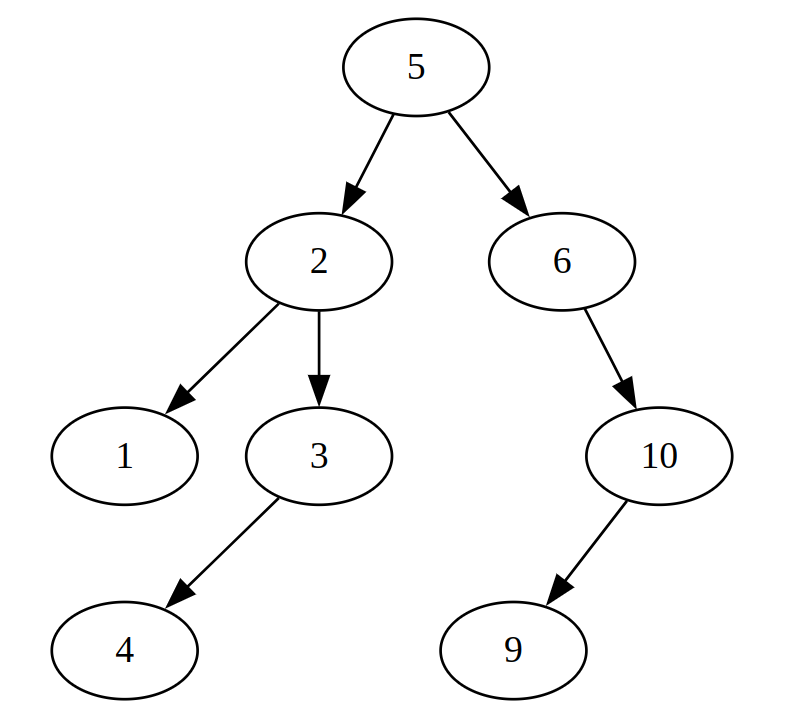
\includegraphics[width=0.35\textwidth]{figs/btree.png} % Adjust width as needed
    \caption{Árvore binária} % Will appear as "Figura 1"
    \label{fig:btree}
    % Your content (e.g., image, diagram, etc.)
\end{figlisting}

O objetivo é analisar as chamadas e usos de funções sobre operações comuns desta estrutura de dados, tais como:

\begin{enumerate}
    \item Percorrimento da árvore em ordem
    \item Uso da Busca em Profundidade, do inglês: \textit{Depth First Search} (DFS)\footnote{
        Algoritmo de exploração de grafos que percorre ramificações até o fim antes de retroceder (backtracking). Usado em árvores, grafos e labirintos – estudado desde o século XIX por Trémaux (\citeauthor{wiki_dfs}, \citeyear{wiki_dfs})\cite{wiki_dfs}.
    }, para obter informações, como:
    \begin{enumerate}
        \item Checar a presença de um determinado nó na árvore
        \item Listar os nós folha da árvore
        \item Percorrer determinado nó até a raiz
        \item Calcular a altura da árvore
        \item Calcular o balanceamento da árvore
    \end{enumerate}
\end{enumerate}

\subsection{Usos}
\subsubsection{Percorrimento em ordem}
Conforme mostrado no Código \ref{listing:abp}, a árvore binária é incializada com uma lista de inteiros totalmente desordenada.
Um dos usos mais comuns da Árvore Binária são os percorrimentos em:
\begin{itemize}
    \item\textbf{Pré-Ordem}
    \item\textbf{Em-Ordem}
    \item\textbf{Pós-Ordem}
\end{itemize}

O percorrimento \textbf{Em-Ordem} pode ser utilizado para percorrer todos os nós da árvore de forma que os nós mais à esquerda são visitados primeiro. Dada a natureza de inserção dos itens em uma Árvore Binária,
sabe-se que os items cujos valores sejam menores estarão à esquerda, ao passo que os maiores à direita. Desta forma, pode-se imprimir a lista totalmente ordenada conforme mostrado no Côdigo \ref{listing:abp-in-order}:

\begin{listing}[H]
    \begin{minted}[linenos,xleftmargin=2mm,tabsize=2,breaklines,autogobble,numbersep=5pt]{python}
    tree.inOrderWalk(lambda node: print(node.value, end=" "))
    # Saída: 1 2 3 4 5 6 9 10 
    \end{minted}
    \caption{Percorrimento em ordem}
    \label{listing:abp-in-order}
\end{listing}

Nota-se no código \ref{listing:abp-in-order} o nível de abstração quando aplicada a programação funcional, pois a medida que o percorrimento ocorre, cada nó encontrado chama a funçåo lambda\footnote{
    Explicar a função lambda
} passada como segundo parâmetro de \textbf{inOrderWalk}. A função então desempenha o papel de imprimir o valor do nó.
Observa-se que ao contrário de simplesmente imprimir o nó, poderia fazer-se qualquer outra operação com o mesmo, como empilhá-los para formar uma nova lista
ordenada, por exemplo.

\subsubsection{Depth First Search (DFS)}

A Busca em profundidade (\textit{Depth First Search}) é um algoritmo que também percorre os nós de uma árvore, assim como o percorrimento em ordem.
Mas diferente de percorrer em ordem, segundo \citeauthor{wiki_dfs}\cite{wiki_dfs}: A Busca em profundidade é uma busca não-informada que progride se
aprofundando tanto quanto possível a partir do primeiro nó filho. Quando a busca chega a um nó folha, retroage-se até o próximo nó e a busca e começa
novamente.
O Código \ref{listing:dfs-percorrer} mostra o percorrimento utilizando DFS.

\begin{listing}[H]
    \begin{minted}[linenos,xleftmargin=2mm,tabsize=2,breaklines,autogobble,numbersep=5pt]{python}
    tree.dfs(lambda node: print(node.value, end=" "))
    # Saída: 5 2 1 3 4 6 10 9 
    \end{minted}
    \caption{DFS: Percorrimento}
    \label{listing:dfs-percorrer}
\end{listing}

Nota-se que o resultado apresentado agora é diferente do percorrimento em ordem apresentado no Código \ref{listing:abp-in-order}.
A busca começa a partir do nó raiz e segue até o último nó folha. Evidentemente, os valores impressos não são exibidos de forma ordenada.

\subsubsection{DFS: Encontrar um nó}

A função passada como argumento para \textbf{dfs} (ao contrário das já apresentadas), espera um valor booleano de retorno.
Este valor é utilizado para controlar quando parar a busca \textbf{dfs}. Caso uma chamada à função passada a \textbf{dfs}
retorne o valor \textbf{True}, a busca é interrompida. Quando \textbf{False}, a busca procede.\linebreak
O Código \ref{listing:dfs-encontra-no-funcoes} mostra a definição de duas funções nas linhas 1 e 2 para serem
utilizadas na \textbf{dfs}:

\begin{listing}[H]
    \begin{minted}[linenos,xleftmargin=2mm,tabsize=2,breaklines,autogobble,numbersep=5pt]{python}
    def retorna_verdadeiro(node: Node): print("Nó visitado:", node); return True
    def encontre_no(node_number: int):
        def closure(node: Node): print("Nó visitado:", node); return node.value == node_number
        return closure
    \end{minted}
    \caption{DFS: Funções de busca}
    \label{listing:dfs-encontra-no-funcoes}
\end{listing}
A função \textbf{retorna\_verdadeiro} apenas exibe o nó visitado e imediatamente retorna \textbf{True}. Enquanto que \textbf{encontre\_no}
retorna uma \textit{Closure}\footnote{
    Explicar closure
}
que compara o nó atual com um valor passado como argumento. Desta forma, \textbf{encontre\_no} se utiliza de DFS para procurar um nó na árvore.\linebreak
Conforme se observa no Código \ref{listing:dfs-encontra-no-verdadeiro}, apenas o nó raiz é visitado quando se usa \textbf{retorna\_verdadeiro}. Isto se deve ao fato de que \textbf{retorna\_verdadeiro} imediatemente retorna
o valor \textbf{True}. Quando uma função retorna \textbf{True}, a \textbf{dfs} retorna o nó atual que está sendo visitado:

\begin{listing}[H]
    \begin{minted}[linenos,xleftmargin=2mm,tabsize=2,breaklines,autogobble,numbersep=5pt]{python}
    tree.dfs(retorna_verdadeiro)
    # Saída: Nó visitado: Node(5)
    # Saída: 
    # Saída: Node(5)
    \end{minted}
    \caption{DFS: retorna\_verdadeiro}
    \label{listing:dfs-encontra-no-verdadeiro}
\end{listing}

No Código \ref{listing:dfs-encontra-no-1} pode-se observar que mais nós são visitados quando se usa \textbf{encontre\_no}. Ao final, depois de percorrer
os nós $(5,2,1)$, o nó $1$ é encontrado e retornado.

\begin{listing}[H]
    \begin{minted}[linenos,xleftmargin=2mm,tabsize=2,breaklines,autogobble,numbersep=5pt]{python}
    tree.dfs(encontre_no(1))
    # Saída: Nó visitado: Node(5)
    # Saída: Nó visitado: Node(2)
    # Saída: Nó visitado: Node(1)
    # Saída: 
    # Saída: Node(1)
    \end{minted}
    \caption{DFS: encontre\_no(1)}
    \label{listing:dfs-encontra-no-1}
\end{listing}

Finalmente, quando um determinado nó não é encontrado, a árvore inteira é percorrida sem que nada seja retornado:

\begin{listing}[H]
    \begin{minted}[linenos,xleftmargin=2mm,tabsize=2,breaklines,autogobble,numbersep=5pt]{python}
    tree.dfs(encontre_no(11))
    # Saída: Nó visitado: Node(5)
    # Saída: Nó visitado: Node(2)
    # Saída: Nó visitado: Node(1)
    # Saída: Nó visitado: Node(3)
    # Saída: Nó visitado: Node(4)
    # Saída: Nó visitado: Node(6)
    # Saída: Nó visitado: Node(10)
    # Saída: Nó visitado: Node(9)
    \end{minted}
    \caption{DFS: encontre\_no(11)}
    \label{listing:dfs-encontra-no-11}
\end{listing}

\subsubsection{DFS: Encontrar nós folha}

O Código \ref{listing:dfs-encontra-folhas} demonstra como obter uma lista dos nós folha usando \textbf{dfs} a partir da árvore.
A natureza do percorrimento \textbf{dfs} é ideal para encontrar tais nós. São encontrados 3 nós de acordo com a linha 3:

\begin{listing}[H]
    \begin{minted}[linenos,xleftmargin=2mm,tabsize=2,breaklines,autogobble,numbersep=5pt]{python}
    leafs: list[Node] = []
    tree.dfs(lambda node: leafs.append(node) if node.left is None and node.right is None else False)
    leafs
    # Saída: [Node(1), Node(4), Node(9)]
    \end{minted}
    \caption{DFS: Nós folha}
    \label{listing:dfs-encontra-folhas}
\end{listing}

\subsubsection{DFS: Nó folha até a raiz}

Uma vez que se tem a lista de nós folha, pode-se utilizar o método \textbf{goToRoot} para saber quais nós estão entre a folha e a raiz.
O Código \ref{listing:dfs-folha-raiz} mostra que os nós $(4, 3, 2, 5)$ formam o caminho entre o nó $4$ (folha), e $5$ (raiz).

\begin{listing}[H]
    \begin{minted}[linenos,xleftmargin=2mm,tabsize=2,breaklines,autogobble,numbersep=5pt]{python}
    tree.goToRoot(leafs[1], lambda node: print(node))
    # Saída: Node(4)
    # Saída: Node(3)
    # Saída: Node(2)
    # Saída: Node(5)
    \end{minted}
    \caption{DFS: Folha à raiz}
    \label{listing:dfs-folha-raiz}
\end{listing}

\subsubsection{DFS: Altura da árvore}

O Código \ref{listing:dfs-altura} demonstra a utilização de composição de funções para calcular a altura da
árvore. Nas linhas 1 a 9 são definidas as funções utilitárias. Por fim, descobre-se na linha 15 que a árvore
tem altura 4.

\begin{listing}[H]
    \begin{minted}[linenos,xleftmargin=2mm,tabsize=2,breaklines,autogobble,numbersep=5pt]{python}
    def pathToRoot(node: Node, tree: BinaryTree):
        arr: list[Node] = []
        tree.goToRoot(node, lambda n: arr.append(n))
        return arr

    def node_paths(lfs: list[Node]): return [ (leaf, pathToRoot(leaf, tree)) for leaf in lfs ]
    def node_length(node: Node, path: list[Node]): return ( node, len(path) )

    tree_heights_pipe = compose_left(
        node_paths,
        lambda arr: [ node_length(node, path) for node, path in arr ],
        lambda arr: [ size for _, size in arr ],
    )

    compose(max, tree_heights_pipe)(leafs)
    # Saída: 4
    \end{minted}
    \caption{DFS: Altura da árvore}
    \label{listing:dfs-altura}
\end{listing}

\subsubsection{DFS: Balanceamento da árvore}

Por fim, tendo-se as informações de altura dos nós folha com a ajuda da função \textbf{tree\_heights\_pipe} (Código \ref{listing:dfs-altura}, linha 9),
pode-se calcular o balanceamento da árvore conoforme mostra a linha 8 do Código \ref{listing:dfs-balanceamento}:

\begin{listing}[H]
    \begin{minted}[linenos,xleftmargin=2mm,tabsize=2,breaklines,autogobble,numbersep=5pt]{python}
    min_height = compose(min, tree_heights_pipe)(leafs)
    diff_height = compose_left(
        lambda arr: tree_heights_pipe(arr),
        lambda arr: [ i - min_height for i in arr ],
        max
    )(leafs)

    print(f"A árvore está { "des" if diff_height > 1 else "" }balanceada")
    # Saída: A árvore está balanceada
    \end{minted}
    \caption{DFS: Altura da árvore}
    \label{listing:dfs-balanceamento}
\end{listing}

Fica evidente que a árvore está totalmente balanceada pois não há nós folha com diferença de altura maior que 1.

\subsection{Implementação}
Conforme visto no Código \ref{listing:abp} (linha 1), a árvore mostrada nos exemplos pertence à bilbioreca \textbf{Btree}
que exporta dois objetos: \textbf{BinaryTree} e \textbf{Node}.\linebreak
A implementação deste módulo consiste em uma estrutura de pastas com três arquivos conforme mosta a Figura \ref{fig:modulo-btree}:

\begin{figlisting}[H]
    \centering
    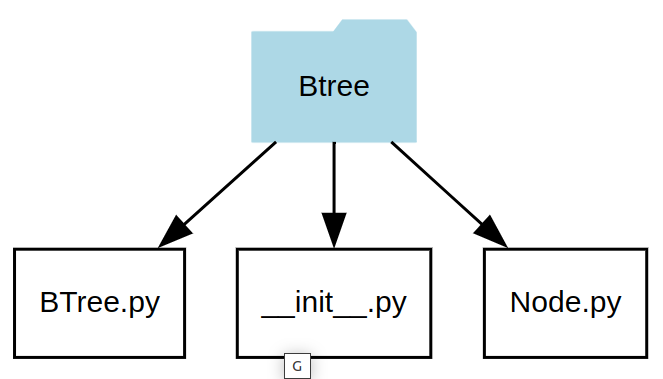
\includegraphics[width=0.35\textwidth]{figs/btree_module.png} % Adjust width as needed
    \caption{Módulo Btree} % Will appear as "Figura 1"
    \label{fig:modulo-btree}
    % Your content (e.g., image, diagram, etc.)
\end{figlisting}

\subsubsection{Node}

A árvore binária é montada com base em seus nós. Um nó é um modelo que representa um dado numérico, contento também
as referências para os nós filhos da direita e esquerda, assim como uma referência ao nó pai.\linebreak
O Código \ref{listing:impl-node} demonstra a implementação do nó:

\begin{listing}[H]
    \begin{minted}[linenos,xleftmargin=2mm,tabsize=2,breaklines,autogobble,numbersep=5pt]{python}
    from typing import Optional

    class Node:
        value: int
        parent: Optional['Node']
        right: Optional['Node']
        left: Optional['Node']

        def __init__(self, value: int):
            self.value = value
            self.left = None
            self.right = None
            self.parent = None

        def __repr__(self): return f'Node({self.value})'
    \end{minted}
    \caption{Node: Implementação}
    \label{listing:impl-node}
\end{listing}

A linha 15 define o método \textbf{\_\_repr\_\_}. Este método retorna um formato de texto que dita como
o nó deve ser exibido quando sua instância é referenciada no notebook, ou quando passada para uma função \textbf{print}.

\subsubsection{BinaryTree}

A implementação de BinaryTree é a árvore em si. No Código \ref{listing:impl-btree-ini} tem-se o método de inserção,
que consiste em inserir os nós filhos na esquerda ou direita a partir da maioridade ou menoridade com o nó pai.

\begin{listing}[H]
    \begin{minted}[linenos,xleftmargin=2mm,tabsize=2,breaklines,autogobble,numbersep=5pt]{python}
    from copy import deepcopy
    from typing import Callable
    from .Node import Node

    class BinaryTree:
        root: Node | None = None

        def __init__(self, arr: list[int]):
            for i in arr:
                self.insert(Node(i))

        def insert(self, node: Node, parent: Node | None = None):
            if self.root is None: self.root = node; return deepcopy(node)
            if parent is None: parent = self.root

            if node.value < parent.value:
                if parent.left is None:
                    node.parent = parent
                    parent.left = node
                    return deepcopy(node)
                return self.insert(node, parent.left)
            
            if parent.right is None:
                node.parent = parent
                parent.right = node
                return deepcopy(node)
            return self.insert(node, parent.right)
        ...
    \end{minted}
    \caption{BinaryTree: Implementação inicial}
    \label{listing:impl-btree-ini}
\end{listing}

\subsubsection{BinaryTree: inOrderWalk}

\begin{listing}[H]
    \begin{minted}[linenos,xleftmargin=2mm,tabsize=2,breaklines,autogobble,numbersep=5pt,firstnumber=28]{python}
    ...
        def inOrderWalk(self, callback: Callable[[Node], None] | None = None):
            def inOrderRecursive(node: Node | None):
                if node is not None:
                    inOrderRecursive(node.left)
                    if callback: callback(deepcopy(node))
                    inOrderRecursive(node.right)

            inOrderRecursive(self.root)
    ...
    \end{minted}
    \caption{BinaryTree: Método inOrderWalk}
    \label{listing:inOrderWalk}
\end{listing}

\subsubsection{BinaryTree: dfs}

\begin{listing}[H]
    \begin{minted}[linenos,xleftmargin=2mm,tabsize=2,breaklines,autogobble,numbersep=5pt,firstnumber=38]{python}
    ...
        def dfs(self, callback: Callable[[Node], bool] | None = None) -> Node | None:
            def _dfs(node: Node):
                if node is None: return
                # print(node)
                if callback:
                    res = callback(node)
                    if res:
                        return node
                if res:=_dfs(node.left): return res
                if res:=_dfs(node.right): return res

            return _dfs(self.root)
    ...
    \end{minted}
    \caption{BinaryTree: Método dfs}
    \label{listing:btree-dfs}
\end{listing}

\subsubsection{BinaryTree: goToRoot}

\begin{listing}[H]
    \begin{minted}[linenos,xleftmargin=2mm,tabsize=2,breaklines,autogobble,numbersep=5pt,firstnumber=51]{python}
    ...
        def goToRoot(self, node: Node, callback: Callable[[Node], None] | None = None):
            callback(node)
            if node == self.root: return
            self.goToRoot(node.parent, callback)
    ...
    \end{minted}
    \caption{BinaryTree: Método dfs}
    \label{listing:btree-dfs}
\end{listing}

% \begin{listing}[H]
%     \begin{minted}[linenos,xleftmargin=2mm,tabsize=2,breaklines,autogobble,numbersep=5pt]{python}
%     \end{minted}
%     \caption{AAAAAAAAAAAAA}
%     \label{listing:AAAAAAAAAAAA}
% \end{listing}